\documentclass[11pt]{article}
\usepackage[margin=0.8in]{geometry}
\usepackage{amsmath,amssymb,booktabs,array,graphicx,xcolor,tikz,hyperref}
\usetikzlibrary{arrows.meta,positioning}
\hypersetup{colorlinks=true,urlcolor=blue,linkcolor=blue}
\setlength{\parindent}{0pt}
\setlength{\parskip}{4pt}
\title{Degree-83 Koblitz factor-base sweep\\Design, replayed artifacts and bounded pilot evidence}
\author{Public known-answer research}
\date{October 9, 2026}
\begin{document}
\maketitle
\textbf{Objective.} Find the factor base and solver configuration with the lowest fully charged index-calculus runtime for one public target. This report distinguishes design coverage, artifact correctness and complete-pipeline performance. A runtime winner requires complete, comparable, verified measurements.

\section*{Exact instances}
The primary curve is $y^2+xy=x^3+1$ over $\mathbf F_{2^{83}}$, using $z^{83}+z^{45}+z^2+z+1$. Its subgroup order is $2417851639230796216685689$, with cofactor 4.

{\small Primary model: \texttt{icv1-f2m83-tm6151469093347-debefd74}\par}

The diagnostic $a=1$ curve has subgroup order $8569786107849059$ and cofactor $1128547018$.

{\small Diagnostic model: \texttt{icv1-f2m83-t6151469093347-cdcc5432}\par}

Both generators and exact encodings are pinned in the exporter and every artifact header. The 81-bit and 53-bit subgroups are separate workloads.

\section*{Finite exhaustive coverage}
The declared design contains 1,050 base specifications and 43,200 solver tuples per base: \textbf{45,360,000 configurations}. Every tuple has a mixed-radix ordinal and one compatibility disposition. Counts sum to the full population, including resource-gated and unimplemented cases. This establishes coverage of the finite design; execution coverage is reported separately. Every other factor base, parameter value, field representation, solver version and heuristic remains outside it.

\begin{tabular}{p{0.23\linewidth}p{0.70\linewidth}}
\toprule
Choice & Declared levels\\
\midrule
Base policies & Sequential, hash-derived and Gray-prefix public x; polynomial, random linear and affine subspaces; 2- and 4-torsion coordinates; Frobenius-invariant module blocks\\
Orbit columns & 32, 64, 128, 256, 600, 900\\
Subspace dimension & 4, 8, 12, 16, 20, 28, 41, 82; invariant-block dimensions 1, 82, 83\\
Closures and seeds & None, sign, signed Frobenius; three frozen public seeds where applicable\\
Summands and splitting & 2--6 summands; 0, 4, 8, 12 split bits\\
Symmetry & None, summand ordering, signed Frobenius, rational 2-torsion, rational 4-torsion\\
Backends & Compact S3 four-sum, MITM, F4, SAT-CDCL, WDSat, Gray FES, Moebius FES, Monica FES\\
Other axes & Binary/Gray order; zero/one/two large primes; 1/4/12 threads; dense or sparse single-word, or BigUint modular LA\\
\bottomrule
\end{tabular}

\section*{Evidence path}
\begin{center}
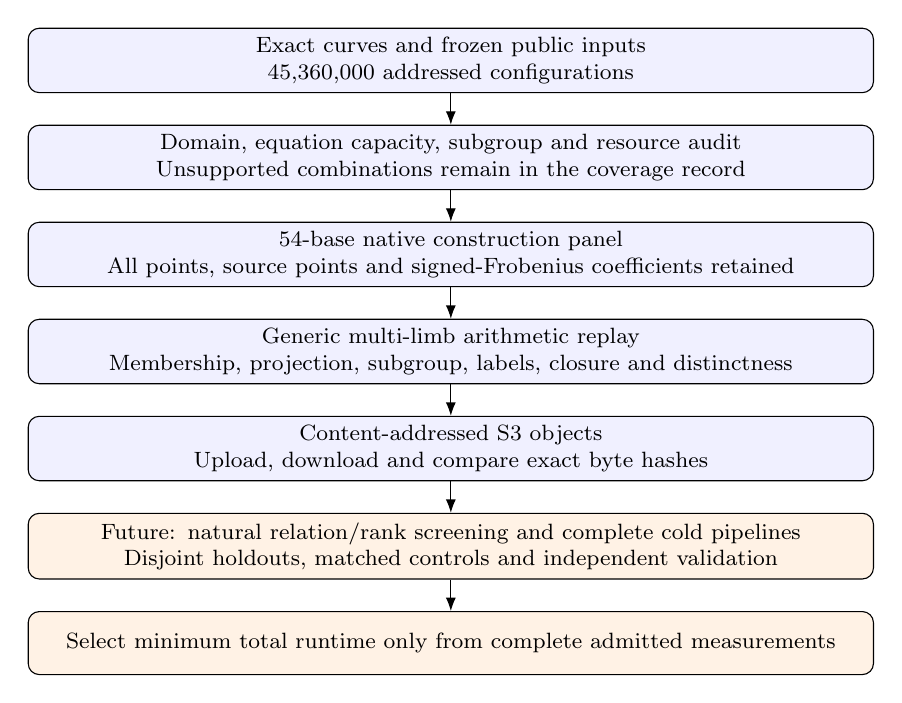
\begin{tikzpicture}[>=Latex,node distance=4mm,box/.style={draw,rounded corners,align=center,text width=10.5cm,minimum height=8mm,font=\footnotesize},future/.style={box,fill=orange!10}]
\node[box,fill=blue!6] (grid) {Exact curves and frozen public inputs\\45,360,000 addressed configurations};
\node[box,fill=blue!6,below=of grid] (gate) {Domain, equation capacity, subgroup and resource audit\\Unsupported combinations remain in the coverage record};
\node[box,fill=blue!6,below=of gate] (base) {54-base native construction panel\\All points, source points and signed-Frobenius coefficients retained};
\node[box,fill=blue!6,below=of base] (replay) {Generic multi-limb arithmetic replay\\Membership, projection, subgroup, labels, closure and distinctness};
\node[box,fill=blue!6,below=of replay] (s3) {Content-addressed S3 objects\\Upload, download and compare exact byte hashes};
\node[future,below=of s3] (full) {Future: natural relation/rank screening and complete cold pipelines\\Disjoint holdouts, matched controls and independent validation};
\node[future,below=of full] (winner) {Select minimum total runtime only from complete admitted measurements};
\foreach \a/\b in {grid/gate,gate/base,base/replay,replay/s3,s3/full,full/winner}{\draw[->] (\a)--(\b);}
\end{tikzpicture}
\end{center}
The construction and replay path supplies exact factor-base artifacts. It does not supply natural relation yield, full rank, an individual logarithm or a total-time winner.

\section*{Structural gate}
Native modular computation gives $\operatorname{ord}_{83}(2)=82$. The nontrivial cyclotomic block in $X^{83}-1$ is irreducible over $\mathbf F_2$. Invariant linear-subspace dimensions are 0, 1, 82 and 83; the small rational-torsion component vanishes under primary cofactor clearing. General subspaces and compact unions of point orbits remain distinct alternatives. A small orbit base is not an invariant linear subspace. The pinned field modulus is checked with the prime-degree irreducibility criterion, using generic polynomial arithmetic.

\section*{Accounting and acceptance}
Cold cost includes curve and base construction, orbit/index setup, relation generation and encoding, every failed attempt, solving and lifting, partial-relation processing, linear algebra, individual logarithm, verification and artifact I/O. Record exclusive intervals and the calibrated operation unit. A missing phase makes the total unknown. Retain timeouts, OOMs, UNKNOWN outcomes and censored completions; none is a win.

The requested runtime comparison needs identical one-target workloads, frozen resource envelopes, A/A controls, at least five interleaved paired rounds, disjoint tuning/holdout targets and a paired 95\% interval outside the admitted noise floor. Use an L2-capable host for wall-time claims. The local Apple M4 Pro host has 14 logical CPUs and 48 GiB of memory, but macOS provides L0 measurement isolation here. Its elapsed construction values are descriptive only. Counted candidates, exact point sets and verification predicates remain valid evidence.

\section*{Pilot population and storage}
The authorized active-process pilot is capped at 3,600 seconds and crosses two curve arms, three public-x policies, three seeds and $K=64,256,600$. All 54 planned bases were constructed. Every complete signed-Frobenius base has $166K$ distinct subgroup points, checked individually by replay. The panel contains 2,748,960 point records, 16,560 orbit-column records and 83,328,324 compressed bytes. Its 54 variants represent 42 distinct point sets; 12 diagnostic sequential/Gray variants duplicate a set exactly. These are artifact counts, not independent experiments.

\begin{center}
\begin{tabular}{rrr}
\toprule
Orbit columns $K$ & Points per base & Bases at this size in full panel\\
\midrule
64 & 10,624 & 18\\
256 & 42,496 & 18\\
600 & 99,600 & 18\\
\bottomrule
\end{tabular}
\end{center}

\begin{center}
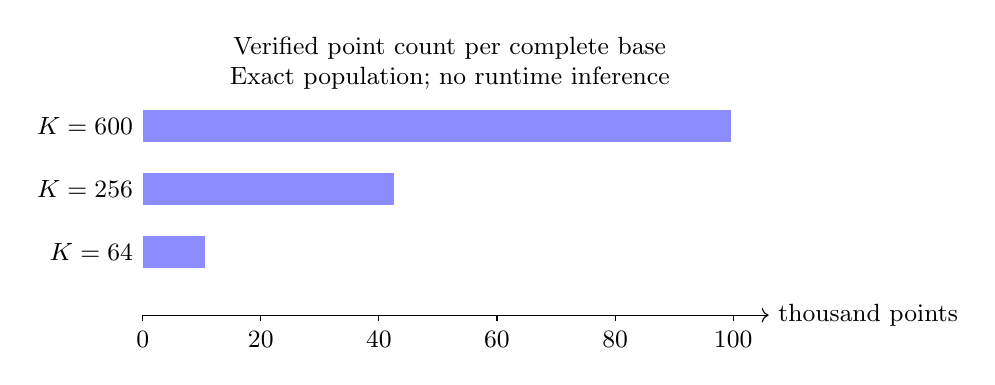
\begin{tikzpicture}[x=0.075cm,y=0.8cm]
\draw[->] (0,0)--(106,0) node[right,font=\small]{thousand points};
\foreach \x in {0,20,40,60,80,100}{\draw (\x,0)--(\x,-0.1) node[below,font=\small]{\x};}
\foreach \y/\v/\lab in {1/10.624/64,2/42.496/256,3/99.6/600}{\fill[blue!45] (0,\y-0.25) rectangle (\v,\y+0.25);\node[left,font=\small] at (0,\y){$K=\lab$};}
\node[align=center,font=\small] at (52,4){Verified point count per complete base\\Exact population; no runtime inference};
\end{tikzpicture}
\end{center}

Full JSONL point sets are gzip-compressed and named by BLAKE3 of the exact compressed bytes, with a separate uncompressed hash and a sorted point-set hash for duplicate detection. The destination is \nolinkurl{s3://crypto-autoresearcher/factor-bases/icv1/etc/} followed by the study, curve arm and content-addressed object path. The uploader requires a matching replay, validates local content, uploads only to this prefix, downloads every object and checks its hash. Manifests and receipts have a separate content-addressed panel path. Generic-versus-wide replay is on the same host and repository; independent-host review remains an additional obligation.

Replay verified 54 bases, 2,748,960 points and 16,560 representatives; S3 matched all 54 objects. Over 1,728 dependent probes, 87,966,720 two-summand lookups found zero relations. Higher-arity yield, rank and full runtime remain unknown.

The separate 53-bit diagnostic arm has three capped cold checks: ordered-pair $K=256$ consumed 606.68 seconds of process wall, ordered-pair $K=64$ consumed 601.32 seconds, and exploratory unordered-pair $K=64$ consumed 600.59 seconds. Each reached its 600-second solver cap with \texttt{UNKNOWN\_budget}; none yielded a completed rank and target record. The unordered $K=64$ index itself completed in 0.771 seconds with 172,640 regular states and 339,776 root-table entries. The ordered runs lack matching phase checkpoints, so the index observation cannot establish a speedup. The recorded construction, replay, probe, upload and cold stages used about 3,530.85 seconds of active execution within the 3,600-second local pilot allowance. The first stage uses an internal timer; the others use process wall. The 81-bit primary arm has no complete cold measurement.

\section*{Prior art and open implementation gates}
The repository has divisor and explicit-orbit bases, torsion-symmetrized systems, F4 splitting, WDSat ANF/capacity tooling, derivative Gray FES, exact single/double-large-prime machinery and the native ecbench accounting harness. Their interfaces have different field, equation and subgroup capacities. The degree-83 primary subgroup exceeds a single word, and the current large-prime field/point adapter is also single-word. FES equation representation and complete verification must cover the full original system; higher-arity chains are not automatically quadratic. WDSat needs sealed source ANF and binary/configuration capacities. Symmetry must preserve the actual domain. Torsion conditions need verification for each coordinate construction.

Cofactor clearing moves x-coordinates outside an input subspace in general. A raw-subspace oracle therefore needs an explicit cofactor-aware lifting and relation equation, including any torsion residue; it cannot simply treat the projected coordinates as unchanged subspace variables. Partial relations must preserve exact modular signs and Frobenius coefficients and be group-checked before cycle filtering. Count graph growth, duplicates, singleton vertices, cycle lengths, matrix density and rank gain, including unsuccessful work.

Historical degree-83 $a=1$ compact-orbit results measured online work after reusable setup. They use a smaller subgroup and a recorded alternative field representation. They do not establish the requested primary cold-cost optimum. Source and historical evidence are pinned in \texttt{PRIOR\_ART.md}. The initial inspected main revision failed before the exporter compiled; the recorded earlier library revision is used for local verification. All actual build and test outcomes, including failures, are retained in \texttt{verification/}.

\section*{Primary literature}
\begin{itemize}
\item Galbraith, Granger, Merz and Petit, \href{https://sacworkshop.org/SAC20/files/preproceedings/18-IndexCalculus.pdf}{On Index Calculus Algorithms for Subfield Curves}: invariant factor-base domains and Frobenius symmetry.
\item Trimoska, Ionica and Dequen, \href{https://arxiv.org/abs/2001.11229}{Parity (XOR) Reasoning for the Index Calculus Attack}: ANF-aware WDSat and branching preprocessing.
\item Bouillaguet et al., \href{https://perso.lip6.fr/Charles.Bouillaguet/static/publis/SAC13b.pdf}{Fast Exhaustive Search for Quadratic Systems in F2 on FPGAs}: derivative Gray enumeration, with explicit equation and hardware assumptions.
\item \href{https://arxiv.org/abs/math/0606607}{Index calculus with double large prime variation for curves of small genus with cyclic class group}: class-group large-prime variation, with transfer to the exact elliptic point representation still an obligation.
\end{itemize}

\end{document}
